% exercise sheet with header on every page for math or close subjects
\documentclass[12pt]{article}
\usepackage[utf8]{inputenc}
\usepackage{latexsym}
\usepackage{multicol}
\usepackage{fancyhdr}
\usepackage{amsfonts}
\usepackage{amsmath}
\usepackage{amssymb}
\usepackage{enumerate}
\usepackage{listings}
\usepackage{graphicx}

% Shortcuts for bb, frak and cal letters
\newcommand{\E}{\mathbb{E}}
\newcommand{\V}{\mathbb{V}}
\renewcommand{\P}{\mathbb{P}}
\newcommand{\N}{\mathbb{N}}
\newcommand{\R}{\mathbb{R}}
\newcommand{\C}{\mathbb{C}}
\newcommand{\Z}{\mathbb{Z}}
\newcommand{\Pfrak}{\mathfrak{P}}
\newcommand{\Pfrac}{\mathfrak{P}}
\newcommand{\Bfrac}{\mathfrak{P}}
\newcommand{\Bfrak}{\mathfrak{B}}
\newcommand{\Fcal}{\mathcal{F}}
\newcommand{\Ycal}{\mathcal{Y}}
\newcommand{\Bcal}{\mathcal{B}}
\newcommand{\Acal}{\mathcal{A}}

% formating
\topmargin -3.5cm
\textheight 22cm
\textwidth 16.0 cm
\oddsidemargin -0.1cm

% Fancy Header on every Page
\pagestyle{fancy}
\lhead{\textbf{Embedded Systems Milestone 7}}
\rhead{ Rafael Dewes (2548365)\\ Kevin M\"uller (2550062)\\ Daniel Schäfer (2549458)}
\renewcommand{\headrulewidth}{1.2pt}
\setlength{\headheight}{110pt}

\begin{document}
\pagenumbering{gobble}
\lstset{language=C++}
%
%\section*{Pins - Scout}
%
%\paragraph{Must not be driven in combination:}
%The only Pins that can not be driven simultaneously are the PINS PD4 and PC5. These PINS are used for the SPI Protocol to select either the ADC and RF module as the "receiver" of a message and only one of the chips can be selected using either Pin PD4 OR Pin PC5.
%
%\paragraph{Must be driven in combination:}
%During the entire process of transferring data using SPI, it is obvious that PB4 has to "run" all the time to ensure that Master and Slaves communicate in a  synchronized manner. To achieve this, data is transferred over the lane with the clock rate given by SCK. Both MOSI and MISO lanes can only be driven when one of the Slave Select Lanes is driven aswell (either PD4 or PC5 in case of scout).
%
%\paragraph{Use-Cases for PINs:} PB4 will pulse continuously with some determined frequency to determine the clockrate with which data is being sent and received over SPI. At the beginning of our application the ATmega board on the scout will mainly communicate with the ADC as its primary job is to find a spot with high brightness to communicate it to the collector. To signal the ADC that sent data is directed to it Pin PC5 will be driven. To achieve communication with the ADC the MOSI lane will be used to request the brightness information of one of the Photoresistors. And the MISO lane will be used to receive this information (coming from the DATA/OUT pin of the ADC).
%
%Whenever the Scout found a spot with a brightness over a certain threshold it will communicate this information to the collector. To do this PD4 will be driven to select the RF module as target of communication over SPI and PD7 will be driven to activate the RF module into TX Mode. Over the MOSI lane PB5 the coordinates will be sent to the RF module which will send these coordinates to the RF module of the collector which will be in RX mode. After receiving the ACK package signaled by pin PD2, the scout will continue searching for a spot with even higher brightness and upon finding one, communicate it to the collector.
%
%The pins PD0 and PD1 might be used for debugging.
%
%\small
%\begin{tabular}{| c || p{30mm} | p{30mm} | p{60mm} |}
%  \hline
%  \textbf{PIN} & FUNCTION & alternate Functions & NOTES\\
%  \hline
%  \hline
%  \textbf{PB4} & I/O Clock of ADC & SCK of RF module & Synchronisation Clock of Serial Peripheral Interface (Master Slave Connection/SPI). Determines the clockrate with which Data is being sent and received over SPI.\\
%  \hline
%  \textbf{PB5} & MOSI lane to ADC & MOSI lane to RF & Master Output, Slave Input lane. The Slave Select lane (PD4/PC5) determines with which of the slaves (either RF module or ADC) the master communicates. This lane is used to communicate to the ADC of which photoresistor data should be read and to communicate information to the RF module.\\
%  \hline
%  \textbf{PB0} & MISO lane to ADC & MISO lane to RF & Master Input, Slave Output lane. The master receives either the output of the data out lane of the ADC or the output of the MISO lane of the RF.\\
%  \hline
%  \textbf{PD4} & RF module Chip Select & - & The Slave Select Lane PD4 detimines that the communication over the BUS is with the RF module (and not with the ADC).\\
%  \hline
%  \textbf{PD7} & RF module Chip Enable & - & Chip Enable Activates RX (used as receiver) or TX Mode (used as transmitter)\\
%  \hline
%  \textbf{PD2} & RF IRQ & - & Maskable interrupt pin. Active low. Confirms either packet arrival when package loaded into RX FIFO (RX mode) or arrival of ACK (acknowledge) packet (TX mode).\\
%  \hline
%  \textbf{PB1} & ADC system clock & - & Prescaled Clock source, which allows time for a conversion to happen inside the ADC (I/O Clock must remain low for at least 36 system clock cycles to allow conversion to be completed)\\
%  \hline
%  \textbf{PC5} & ADC Chip Select & - & The Slave Select Lane PC5 detimines that the communication over the BUS is with the ADC (and not with the RF Module).\\
%  \hline
%  \textbf{PD0} & Dev Port RX & - & Communication Input of UART Serial Communication (Output atmega328 - Input Dev Port)\\
%  \hline
%  \textbf{PD1} & Dev Port TX & - & Communication Output of UART Serial Communication (Output Dev Port - Input atmega328)\\
%  \hline
%\end{tabular}
%\normalsize
%
%\vspace{1cm}
%
%\newpage
%\section*{Pins - Collector}
%
%
%\paragraph{Must not be driven in combination:}
%All pins mentioned on the cheatsheet can be driven in combination.
%
%\paragraph{Must be driven in combination:}
%During the entire process of transferring data using SPI, it is obvious that PB0 has to "run" all the time to ensure that Master and Slaves communicate in a  synchronized manner. To achieve this data is transferred over the lane with the clock rate given by SCK. Both MOSI and MISO lanes can only be driven when one of the Slave Select Lanes is driven aswell (in the case of collector, this is only PB3 as only one slave is specified on the cheatsheet)
%
%\paragraph{Use-Cases for PINs:}
%
%The Collector will set the RF module to RX mode using PC7 and listen for a coordinate sent by the scout. An interrupt on PD2 signalizes receiving a coordinate sent by the scout. The data packet which contains the coordinate will be transferred from the RF module to the atmega over PD7, the MISO lane. Communication over SPI with the SPI module always drives pin PB3 and PB0 will be driven in a set frequency to determine the clock rate with which data is being sent and received over SPI.
%
%The pins PD2 and PD3 might be used for debugging.
%
%
%\small
%\begin{tabular}{| c || p{30mm} | p{30mm} | p{60mm} |}
%  \hline
%  \textbf{PIN} & FUNCTION & alternate Functions & NOTES\\
%  \hline
%  \hline
%  \textbf{PB0} & RF SCK &  & Serial Clock given by master to synchronize communication over SPI protocol. \\
%  \hline
%  \textbf{PD5} & RF MOSI &  & Master Output - Slave Input lane used for SPI. This lane will e.g. be used to send package contents to the RF chip.\\
%  \hline
%  \textbf{PD7} & RF MISO &  & Master Input - Slave Output lane used for SPI. This lane will e.g. be used to receive package contents from the RF chip.\\
%  \hline
%  \textbf{PB3} & RF chip select &  & This Slave Select Lane detimines that the communication over the BUS is with the RF module\\
%  \hline
%  \textbf{PC7} & RF chip enable &  & Chip Enable Activates RX (used as receiver) or TX Mode (used as transmitter) \\
%  \hline
%  \textbf{PD2} & RF IRQ & Dev Port RX & Maskable interrupt pin. Active low. Confirms either packet arrival when package loaded into RX FIFO (RX mode) or arrival of ACK (acknowledge) packet (TX mode). Additionally this lane is the communication Input of UART Serial Communication (Output atmega32u4 - Input Dev Port) \\
%  \hline
%  \textbf{PD3} & Dev Port TX &  & Communication Output of UART Serial Communication (Output Dev Port - Input atmega32u4) \\
%  \hline
%\end{tabular}
%\normalsize
%
%\newpage
%\section*{Interrupts}
%\subsection*{Scout (3pi/ATmega 328):}
%\begin{itemize}
%\item \textit{Finding a location where the photo sensor readings surpass 200 (external)}\\
%The sensors' readings get to the ADC. After checking against the threshold, we send the value to the Controller. A pin change interrupt is triggered at pin PB0, where we need to save the coordinates. We then communicate them to the Collector with the RF module. The PD4 pin allows us to access the RF chip, the MOSI pin is used to get the coordinate data to the communication module, so during this process we cannot access the ADC. We also need Pin PD2 from RF IRQ to control for sent acknowledgement, where the RF module sends its interrupts regarding receive, transmit, transmit fail.
%\item \textit{Check for timer $> 5$ minutes (internal)}\\
%We need to fire an interrupt after a 5 minute time limit and send the saved coordinates to the Collector. This happens internally such that we do not have to drive a pin. We must pay attention to the overflow as 5 minutes are relative to our system clock. 
%Afterwards we need to signal coordinates to the Collector as we do in the above case, so at least MOSI and PD2 are used.
%
%\end{itemize}
%After an interrupt, the program counter is pushed on the stack; after the interrupt routine it is popped back from the stack.
%There are multiple Timer/Counter Interrupt Vectors we can (and probably must) use for the 5 minute timer.
%(TIMER0 COMPA and TIMER0 OVF can control the timer overflow.)
%For the 3pi robot we have a minimum response time of four clock cycles for interrupt handling. 
%
%\subsection*{Collector (Zumo/ATmega 32u4):}
%\begin{itemize}
%\item \textit{Check if communication by Scout $\neq -1$ (external)}\\
%We wait for coordinates sent by the Scout. When coordinate data is received through the communication, the RF module will send an interrupt on IRQ pin to pin PD2 on ATmega 32u4. We can request the coordinates via RF MISO (PD7) after we select the RF chip (PB3). Now we need to handle the received coordinates over the MOSI (Pin PD5). 
%\item \textit{Other robot in specified proximity sensor range (external)}\\
%After the proximity sensor reads a value below the predetermined threshold, it puts the signal through to the Controller. Here we get an interrupt, which in turn leads to changing the orientation of our collector robot to the direction of sensed object. 
%\end{itemize} 
%
%
%The interrupt response time for the Zumo robot is at minimum five clock cycles.

%
%\textit{How does the interrupt service routine handle the interrupt? Which pins are affected?} \\
%
%3pi/Scout(ATmega 328): \\
%\begin{itemize}
%\item Finding a location: INT0, 0x0002
%The interrupt is executed asynchronously 
%\item Check for timer: TIMER2 COMPA, 0x000E 
%\end{itemize}
%Zumo/Collector(ATmega 32u4): \\
%\begin{itemize}
%\item Check Scout communication: INT0, \$0006
%\end{itemize}
%
%\textit{Which conditions should an interrupt concerning the communication with the expansion board occur?} \\
%\textit{Is the interrupt triggered by an external or internal source?} \\

%
%\newpage
%\section*{Hybrid Automata}
%\subsection* {Scout}
%The scout has two modes of operation: Moving in the dark (areas with photo sensor readings $\leq 200$) and light areas (areas with photo sensor readings $> 200$). The input sensor readings are in the variable photoSignal. In both states, position and angles are modelled as derivates calculated from the left and right angular wheel velocities u\textsubscript{l} and u\textsubscript{r}. For simplicity, we modelled the wheels in a way that they can either turn forward or backward with constant speed of 1. We also introduced continuous variables for the harvesting positions which are only updated in the state MoveInLight. Before that, they remain at $-1$. Those variables as well as the angular wheel velocities are also the output variables. The self-loop in MoveInLight updates the variable bestP with the best photo sensor reading so far. From the exercise we were not sure whether this best value should only include values $> 200$ or all values. If we would want all values we would have to add such a self-loop in the MoveInDark state. Another continuous variable clock keeps track of the time and triggers a transition to state Done after 300 seconds where the best harvesting position read so far will be output.\\
%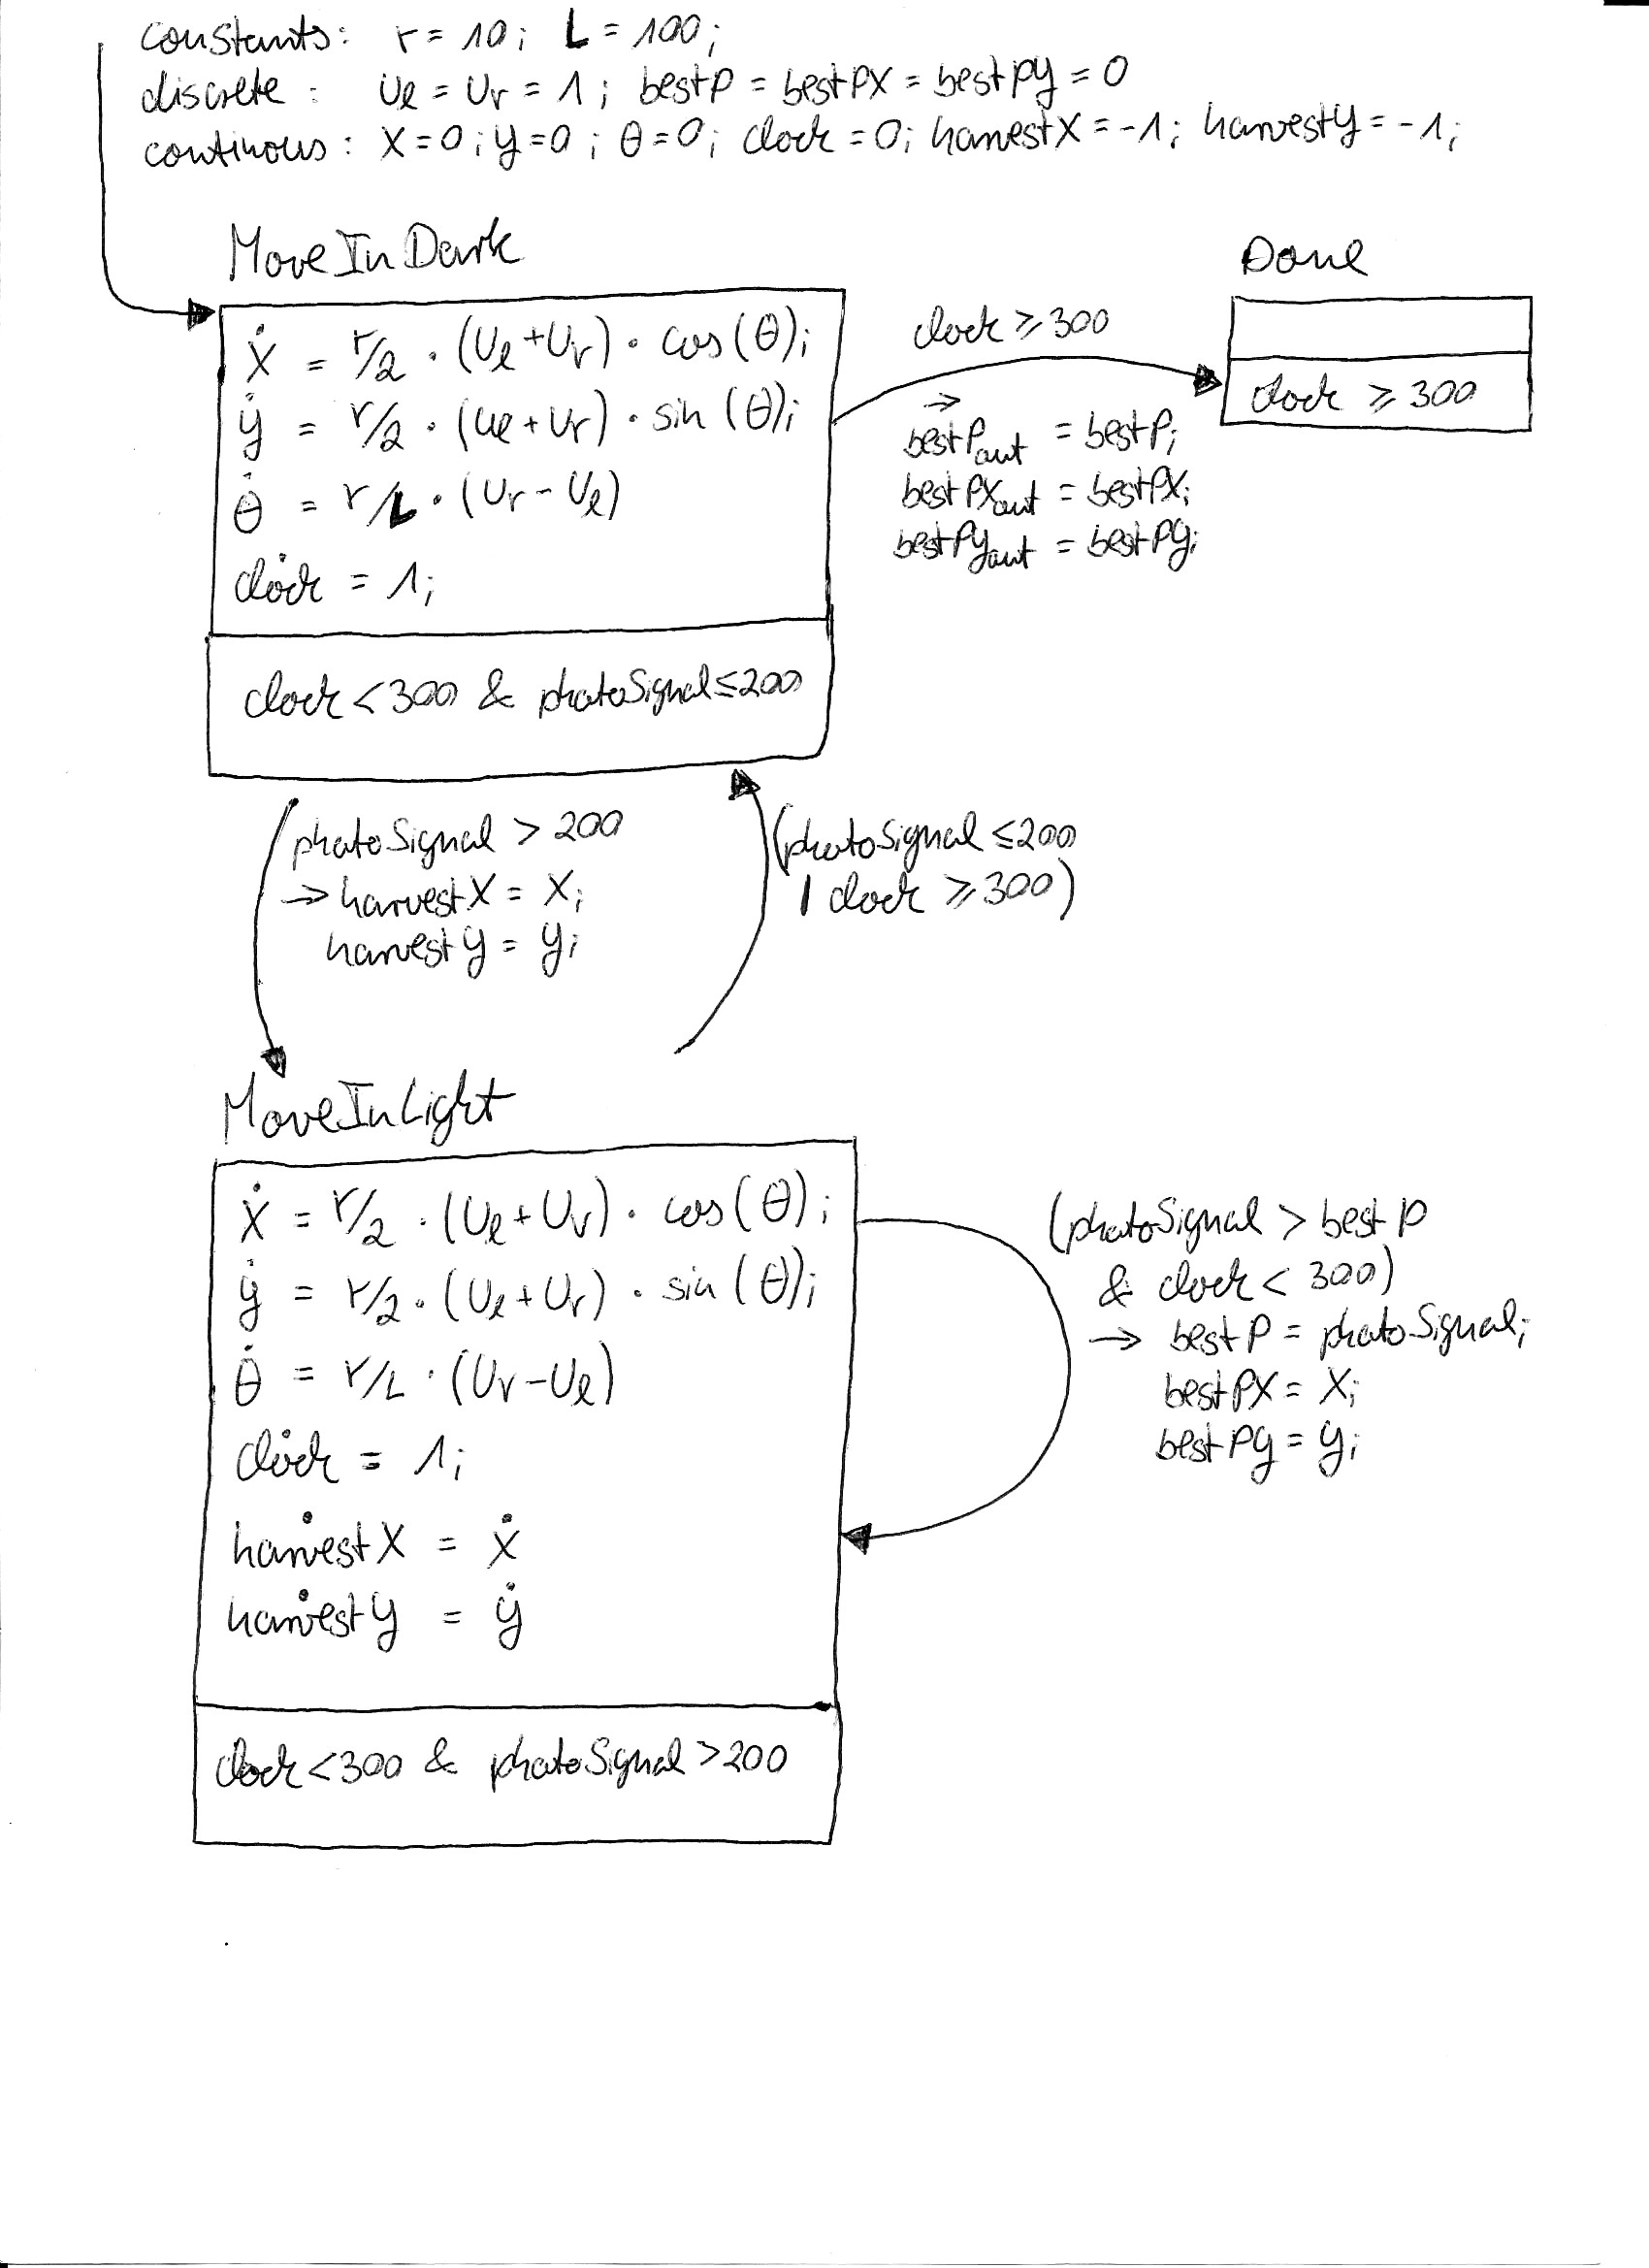
\includegraphics[scale = 0.8]{pictures/hybrid_automata_scout}
%
%\subsection* {Collector}
%The collector has two main states: Annoy and Harvest. Input variables are harvestX and harvestY which it gets from the scout and pLeft, pFront and pRight which are the left, front and right proximity sensor readings. In the initial state Annoy, the collector drives forward and turns left or right when the proximity sensors at the sides indicate a nearby object. This is achieved by inverting the angular wheel velocitys, e.g. in order to turn left, we flip u\textsubscript{l} from 1 to -1. Just as for the scout, u\textsubscript{l} and u\textsubscript{r} are our motor control output signals. In the turning state we only have to update $\Theta$ because the robot is not moving forward but only rotating at the same position. Once a harvest signal is received by the scout, the robot transitions to the Harvest state. There, it computes the angle to which it has to turn in order to point to the harvesting position. The function \verb!getAngle()! calculates the required angle:
%\begin{lstlisting}
%getAngle(x, y, harvestX, harvestY) {
%    vec = (harvestY- y, harvestX - x);
%    angle = arctan(vec.y / vec.x);
%    if (vec.x < 0) 
%        angle += 180;
%    if (angle > 180) 
%        angle = -360 + angle;
%    if (angle < -180) 
%        angle = 360 - angle;
%    return angle;
%}
%\end{lstlisting}
%The robot compares this angle with its current angle $\Theta$  and transitions into either TurnLeft or TurnRight and turns until it points straight at the harvesting position. It then transitions back into the Harvest state where it moves forward towards the harvesting position. Once there, it stops. To ensure that the system does not transition back to Annoy once it has been in Harvest, we introduced the variable a that ensures that states TurnLeft and TurnRight can only transition to the states that transitioned to them and, in particular, not from Harvest to Annoy or vice versa.\\
%Note that the turning functionality as we have modelled it for the collector can work in the same way for the scout. For simplicity we have omitted it in the above automaton because given the assumption from the exercise that we have an infinitely large map with no sensible boundaries it does note make a difference whether the scout makes turns or only keeps driving forward. We have also modelled both automata in Stateflow where we let the scout make turns based on the current clock value.\\
%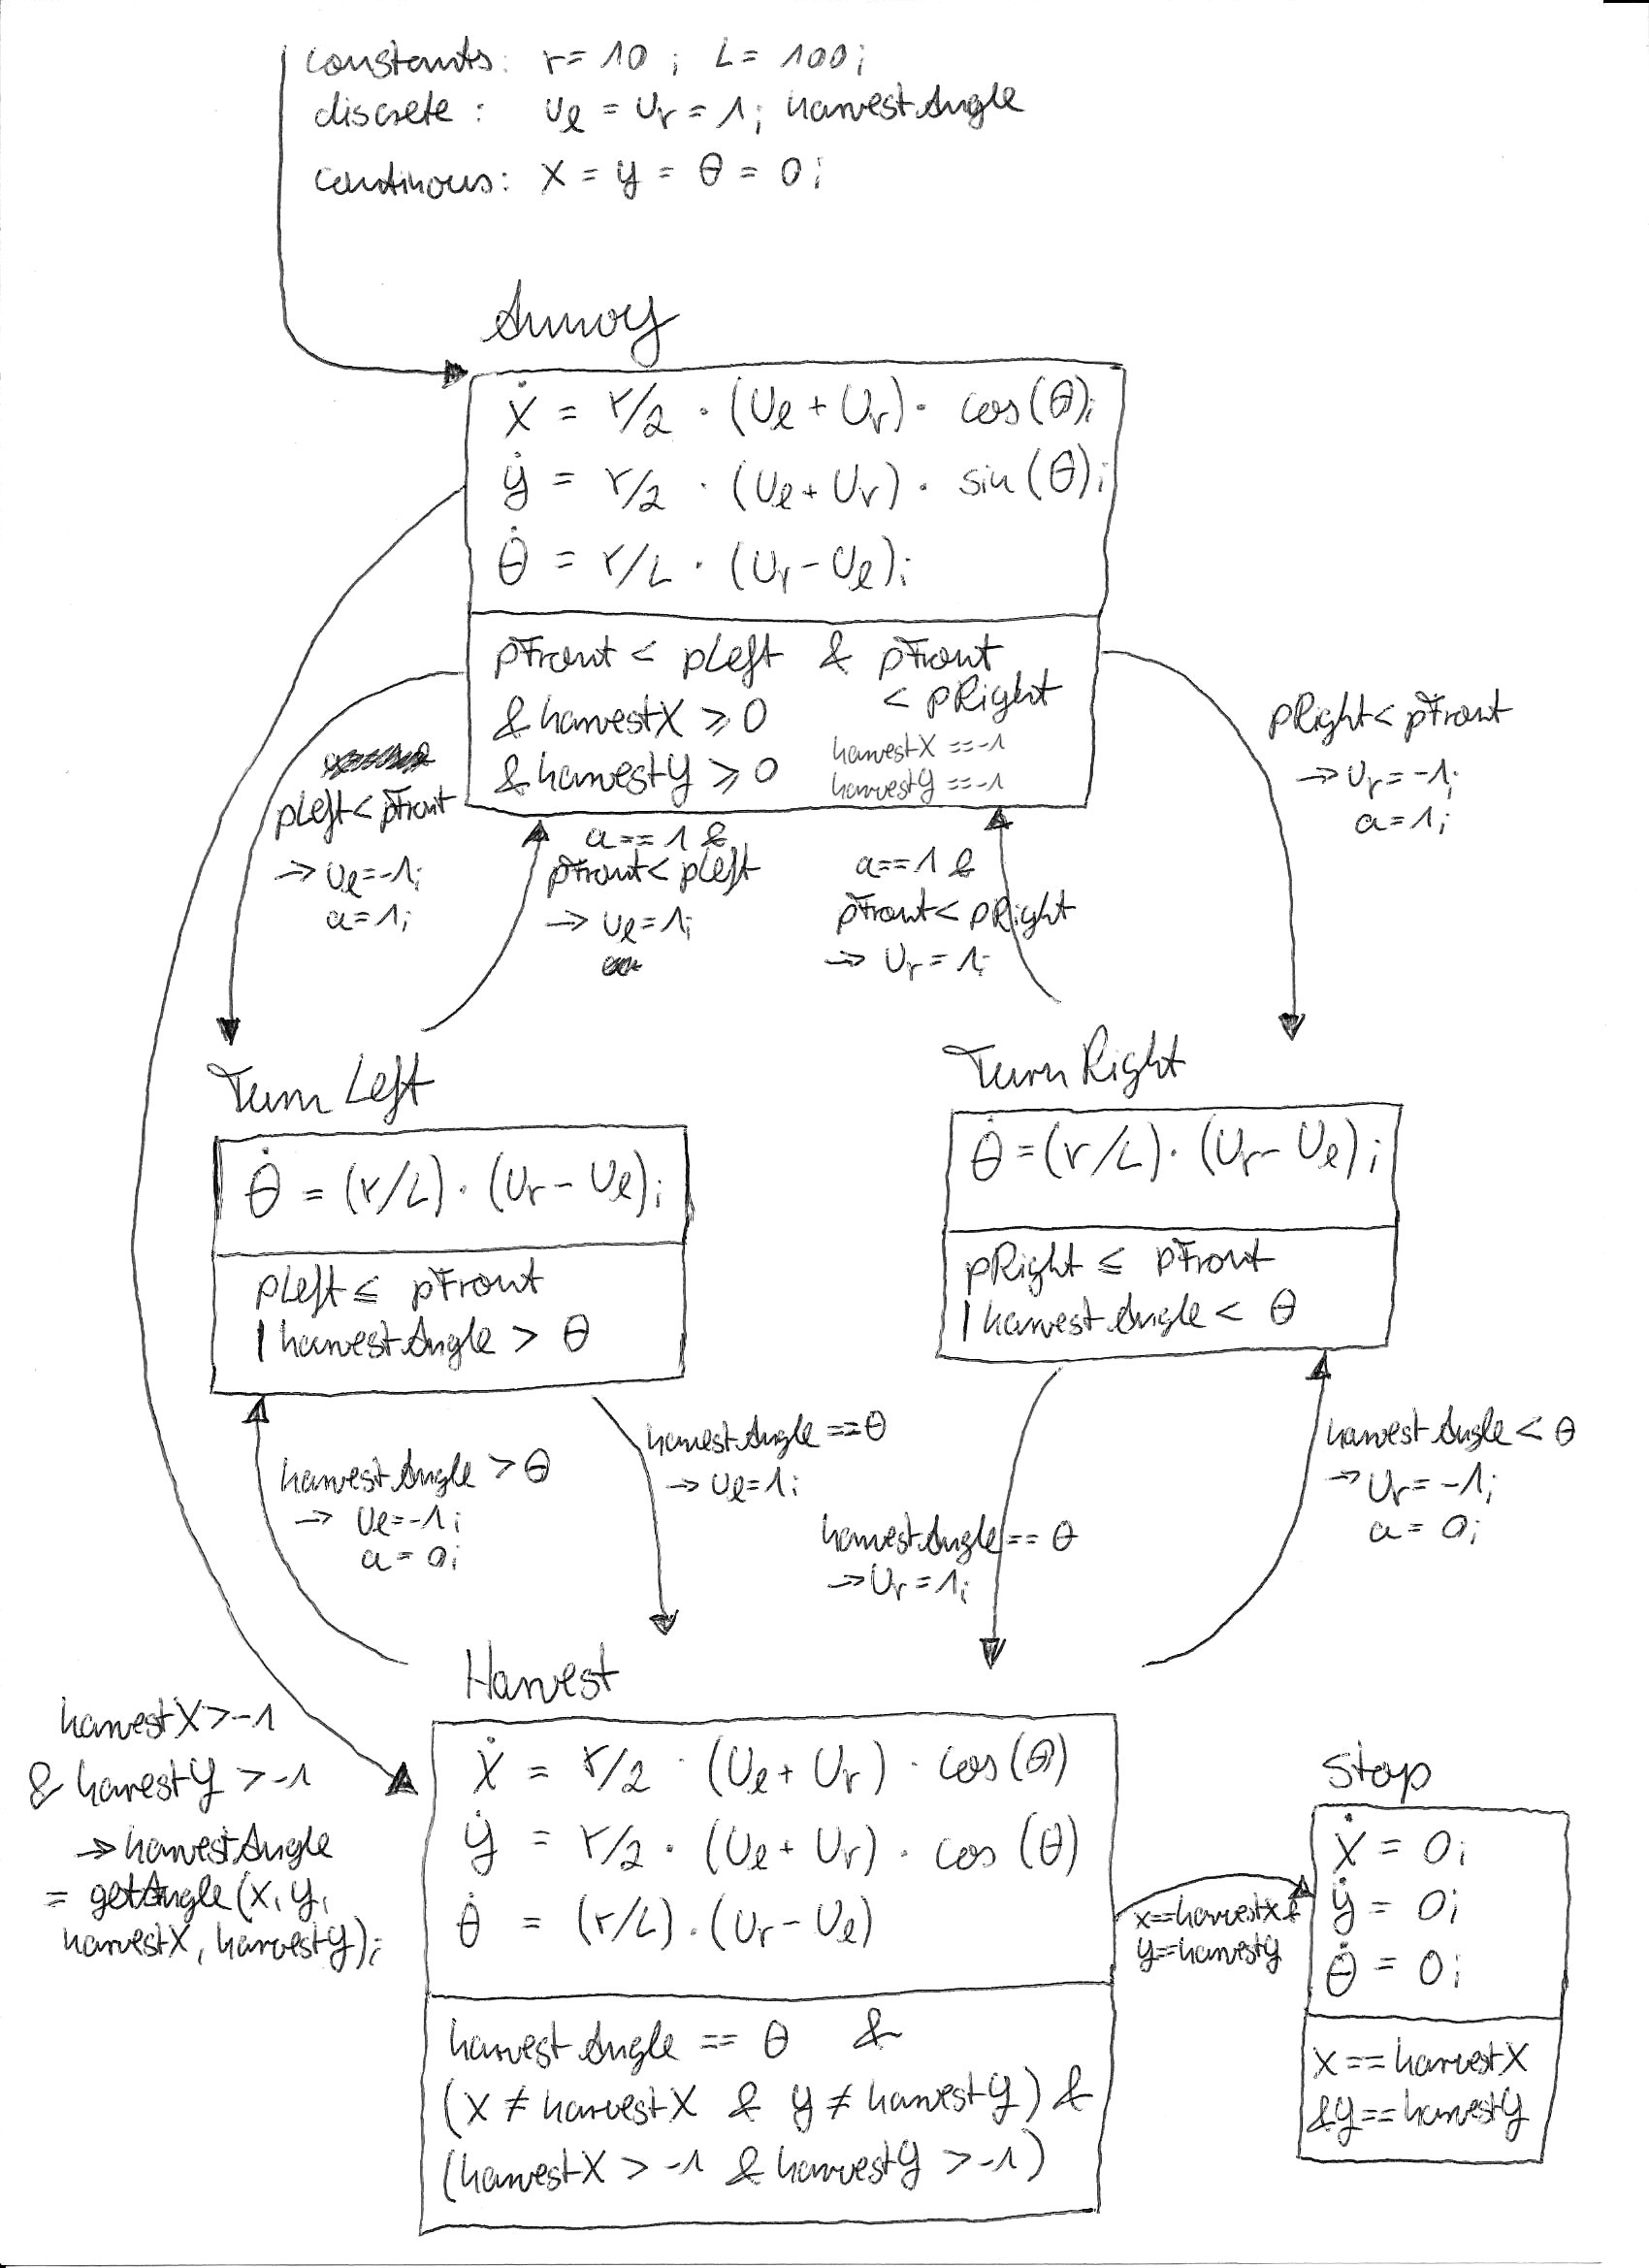
\includegraphics[scale = 0.8]{pictures/hybrid_automata_collector}


\end{document}
